\chapter{Theory}
\label{chap:Theory}

\section{Introduction}
This chapter will provide an explanation of different types of concepts that is essential to understand before reading the rest of the thesis. It will cover various forms of software testing, multiple techniques of security testing, and other relevant information deemed necessary to understand the thesis.


\section{Software Development Lifecycle}
\acrlong{sdlc} can be defined as \textit{"structured process that enables the production of high-quality, low-cost software, in shortest possible production time. The goal of the \acrshort{sdlc} is to produce superior software that meets and exceeds all customer expectations and demands"}\cite{sdlc1}.  SDLC consists of several phases that provide a framework for software development testing and deployment. Below are the six phases that fulfill the \acrshort{sdlc}. 

\subsection{Planning} 
The planning phase is the first phase of the \acrshort{sdlc}. During this phase, the project's goals and objectives are determined. Aspects like resources, costs, and time should be discussed, and a timeline for the work should be created.  Furthermore, a project plan should be developed where tasks and resources necessary to construct the project's structure are identified, prioritized, and assigned. \cite{planningphase}
 
\subsection{Implementation}
It is in this phase the actual development of the software takes place. During the implementation phase, the software design is translated into code using programming languages. After the code is completed and reviewed, the building process begins, and several security scans are performed.
The implementation phase is considered quite important since this is the phase that involves the actual development of the software and the preparation of the software for deployment into the environment.  \cite{ImplementationSDLC}
 
\subsection{Testing}
In this phase, the development team ensures that the software meets the functional, performance, and quality requirements that were decided in the earlier phases of the \acrshort{sdlc}. Here the software gets tested so that any potential defects get identified and corrected. It is in this phase the developer team ensures the high quality of the software and that it meets the needs of the users. \cite{TestingSDLC}
 
\subsection{Deployment}
In the deployment phase, the process of releasing the software into the environment can be considered the main priority. In this phase, the deployment team works together with the development team and other stakeholders to plan the release of the software so that it goes as smoothly as possible. This also includes creating the deployment timeline, selecting a method for the deployment, and defining the environment the software is being deployed into. \cite{DeploymentSDLC}

\subsection{Maintenance} 
In this phase, the software has been deployed and is now being monitored to ensure that it is functioning as it was designed to. Any refactoring and upgrades are done if needed. Monitoring the software can be done in different ways depending on how the maintenance phase has been set up. The most common way of monitoring however is usually through real-time reporting or ad-hoc reporting systems, which are automatically generated within the software that was created and then sent to the company that created it.\cite{MaintenanceSDLC} 

\begin{figure}[H]
    \centering
    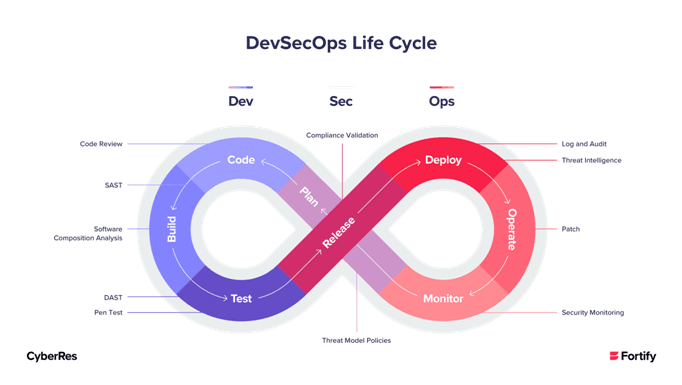
\includegraphics[width=0.8\columnwidth]{Images/devsec.png}
    \caption{DevSecOps Life Cycle}
    \label{fig: DevSecOps Life Cycle}
\end{figure}


\section{Functional Testing vs Security Testing}
Software testing is a very broad area, and each test varies according to its purpose or process - but the primary goal of software testing is to verify the quality of software systems through planned and structured testing under controlled conditions. Functional testing is emphasizing the software's behavior and that the software is working as expected. The functional test cases are based on the requirements of the software which were specified by the stakeholder. There are several functional testing methodologies that can be conducted, such as unit testing and integration testing. White box testing and black box testing are some examples of security testing methods. This topic will be described more in section  \ref{boxtesting}. 
\cite{difftesting} 
Unit testing involves testing small components of the code, which is known as units to determine if the units behave as expected. These tests are typically executed early in the \acrshort{sdlc} to identify bugs early on and save time in the rest of the process. The goal of the unit testing is to run tests on all possible components in an isolated test environment to confirm if the code operates as anticipated. Integration testing, on the other hand, evaluates how the previously tested components perform when integrated into a larger system and communicate across various components. 
\cite{unitvsintergration}

Security testing, on the other hand, wants to break the software to uncover vulnerabilities. The testing aims to identify all possible weaknesses that attackers might exploit. During the testing, the testers perform the test from the attacker's point of view. These kinds of tests can be done manually or be done by software tools, called automated security testing tools. The goal of evaluating security functionalities is to verify if protective measures like authentication are functioning as expected. Security testing will also try to simulate attacks on the software and determine its capability to defend against them.\cite{whysectest}



%Introduction


\section{Application Security Testing}
Application Security Testing can be described as "\textit{process of making applications more resistant to security threats, by identifying security weaknesses and vulnerabilities in source code.}\cite{AST}

Below are some of the different security tools that can be used to make applications more resistant to security threats, and which the group will use in securing the \acrshort{sdlc}. Box testing is also mentioned which is a type of testing technique that the different tools use for testing.  
\newpage
\subsection{Box testing}
\label{boxtesting}

\subsubsection{Black Box Testing}
Black box testing mainly focuses on the functionality and behavior of the application without knowing the structure and processes within it. One can imagine the application being a black box, not being able to see what's inside, but only focusing on the resulting output from the given input. The software will pass the black box test if the input gives the expected output. \cite{blackbox}

\subsubsection{White Box Testing}
White box testing focuses on the application from within. In such tests, the source code and infrastructure will be looked at. The testing consists of covering paths, statements, and branches, among other things. A white box tester looks for security holes by testing the code and therefore requires to have knowledge of programming and IT. The tester looks through the code to find weaknesses such as infinite loops or data flow issues. However, white box testing can be quite complex and when running such testing on a large amount of code, it can take days to test.   \cite{whitebox}

\subsubsection{Grey Box Testing}
Grey box testing is a method that limits the user's knowledge of the different components being tested. It is a combination of white box testing and black box testing, where the user has access to internal code or design but not enough access to run a full white box testing, and the test practices are done at the same level as black box testing. \cite{GreyBox}


\subsection{SAST}
\acrlong{sast} is white-box testing that analysis the source code of an application to identify security vulnerabilities within the code. This method of testing usually takes place during the development phase of the \acrlong{sdlc}. The primary purpose of this method is to identify and remediate security issues before the application actually is deployed. \cite{sast}

\acrshort{sast} tools scan source code for known security threats, such as \gls{Cross-site scripting}, \gls{SQL-injection}, and \gls{Buffer-Overflow}. \acrshort{sast} tools also give warnings on any security weaknesses that may lie in the code that potentially can be exploited. After the tool has gone through the code it generates a report that contains the different vulnerabilities that it has identified, including a more in-depth description of the vulnerability and remediation on how to fix it. \acrshort{sast} usually runs white box testing  which is mentioned in section 2.4.1.2. 

One of the advantages of \acrshort{sast} is that it gives detailed information about the source of the vulnerability, which gives the developer a better understanding of how to fix the issue. 

There are, however, some limitations to \acrshort{sast} tools. For example, it can only detect vulnerabilities that are present in the source code. This means that it cannot detect vulnerabilities that result from the interaction between different components of an application.
\\
\begin{figure}[H]
    \centering
    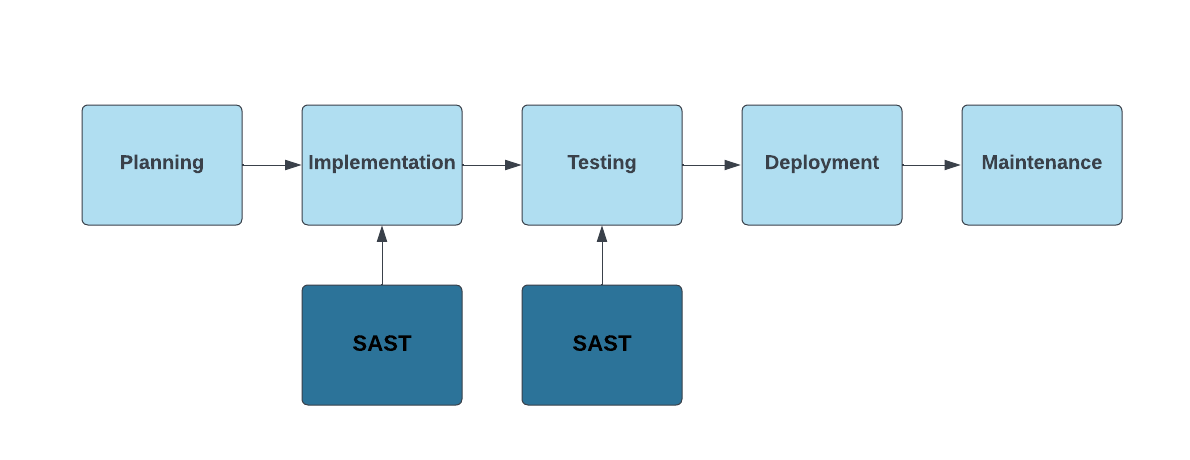
\includegraphics[width=0.8\columnwidth]{Images/sast.png}
    \caption{Where to perform SAST in SDLC}
    \label{fig: Performance of SAST in SDLC}
\end{figure}


\subsection{DAST}
Compared to \acrshort{sast}, \acrlong{dast} is black-box testing. The purpose of \acrshort{dast} is that it evaluates the security of an application by performing security assessments of a running instance of the application. Unlike \acrshort{sast} which analyzes the source code of an application, \acrshort{dast} evaluates the application as its being used, this includes the interaction of different components and the runtime environment. 

\acrshort{dast} simulates real-world attacks, which is done by sending malicious requests and inputs to the application it is testing and then monitoring the responses. In the end, the tool generates a report that includes the different vulnerabilities that were identified, including a more in-depth description as well as remediation on how to fix the issue. 
\acrshort{dast} usually runs black box testing  which is mentioned in section 2.4.1.1. \cite{dast}

An advantage with \acrshort{dast} is that it can identify security issues that are not detectable through \acrshort{sast}, this can for example be interactions between different components. Another advantage is that with \acrshort{dast}, it can identify different vulnerabilities that get triggered, for example when the application is under heavy load or when are specific inputs received.

However, there are some limitations with \acrshort{dast} as well, one being that it can only detect vulnerabilities that are present in the deployed version of the application and cannot give an in-depth description of vulnerabilities that lie in the source code.
\begin{figure}[H]
    \centering
    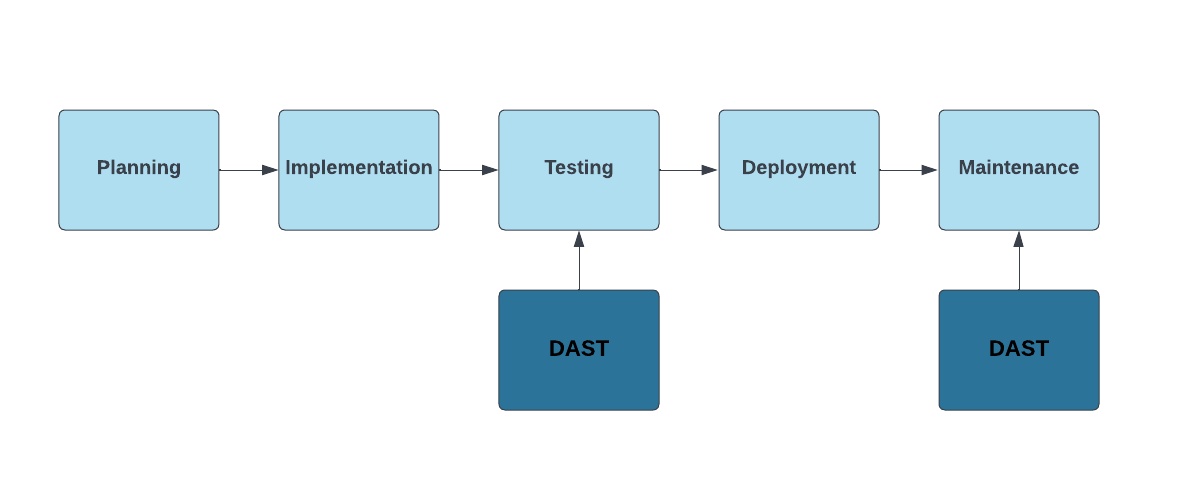
\includegraphics[width=0.8\columnwidth]{Images/dast.png}
    \caption{Where to perform DAST in SDLC} 
    \label{fig: Where to perform DAST in SDLC}
\end{figure}



\subsection{SCA}
\acrlong{sca} is a type of software security testing tool that analyzes the dependencies of a software application to identify and manage potential security risks. The main objective of the \acrshort{sca} is to identify third-party components that may contain security vulnerabilities. \cite{sca}

 \acrshort{sca} scans the application's code to identify all of its \gls{dependency}, including the different versions of the components used. It then cross-references these \gls{dependency} to different databases that include known vulnerabilities and then generates a report containing any potential risk. In comparison to the others, the report also includes an in-depth description of the vulnerability as well as a recommendation to update the components to newer versions or replace these. \acrshort{sca} usually runs grey box testing  which is mentioned in section 2.4.1.3. 

An advantage with \acrshort{sca} is that it can quickly identify risks that may be introduced from third-party components. It is rather common that modern applications rely on a large number of different dependencies, which therefore make \acrshort{sca} useful. It can provide a comprehensive view of the security risks associated with an application and help developers make informed decisions about the security and their applications. 

However, it is important to remember that \acrshort{sca} does not always have access to updated information, and may give some false positives about vulnerabilities that don't necessarily exist anymore. 
\\
\begin{figure}[H]
    \centering
    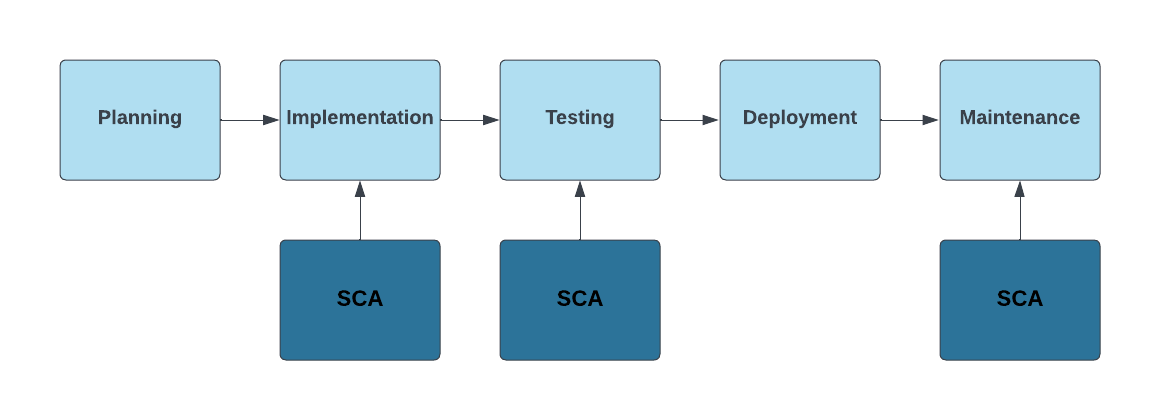
\includegraphics[width=0.8\columnwidth]{Images/sca.png}
    \caption{Where to perform SCA in SDLC} 
    \label{fig: Where to perform SCA in SDLC}
\end{figure}

\newpage
\subsection{Comparison of SAST, DAST, and SCA}
Upon reviewing the different security application tests, similarities between \acrshort{sast}, \acrshort{dast} and \acrshort{sca} were discovered. The table below shows some commonalities, which indicates that a combination of the different testing mechanisms can enhance the testing process of the application. 
\begin{figure}[H]
    \centering
    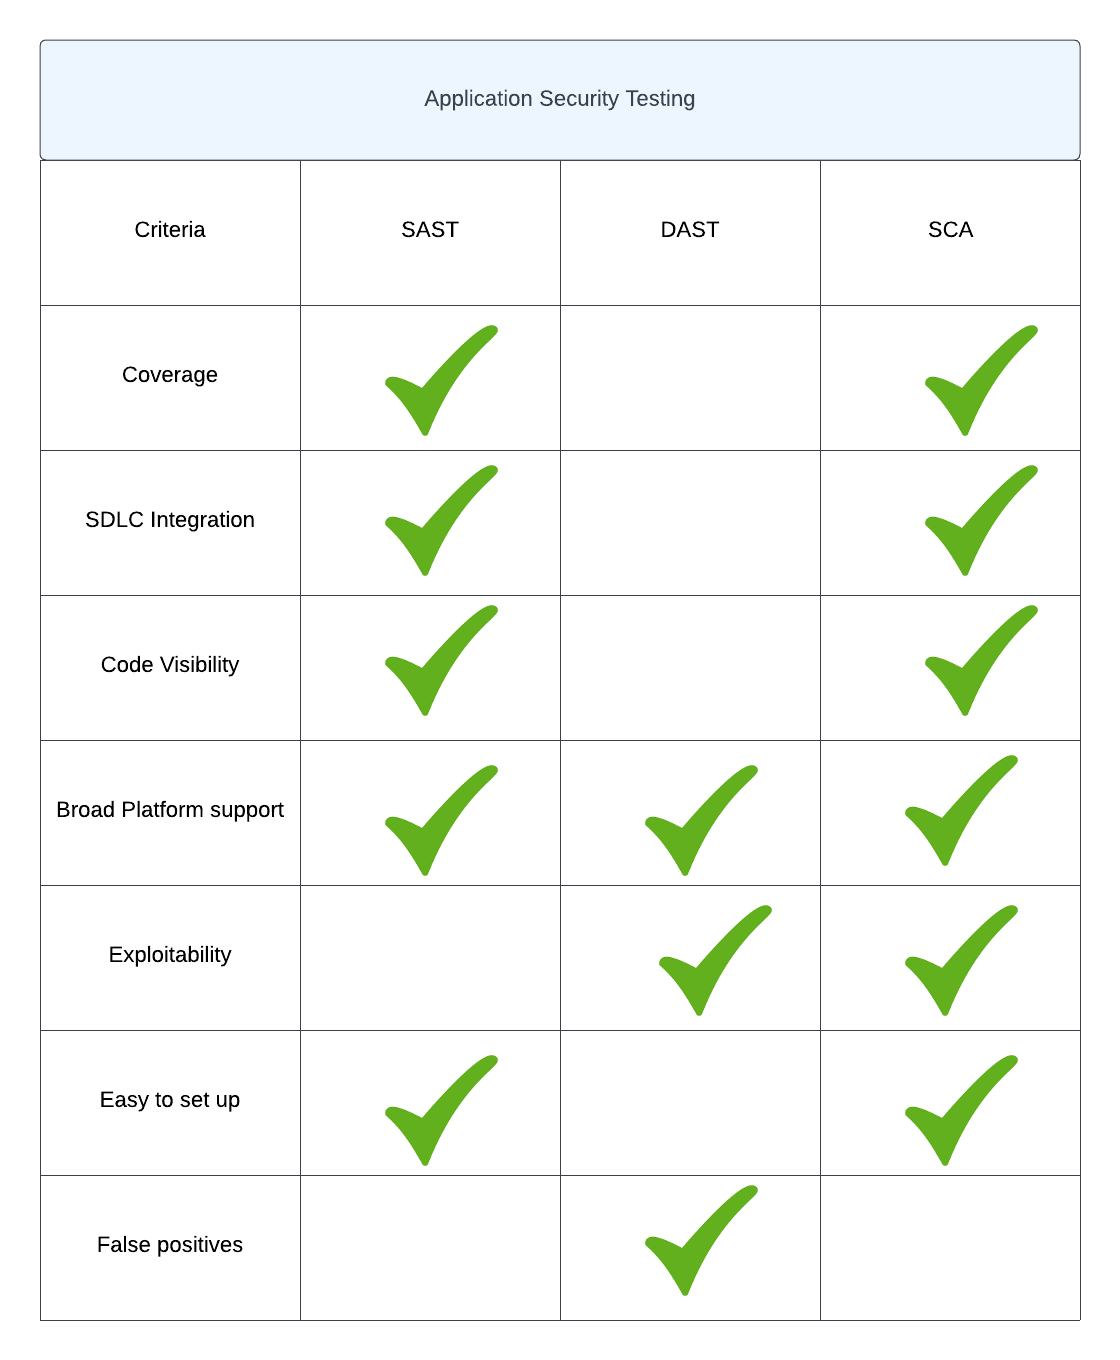
\includegraphics[width=0.8\columnwidth]{Images/ApplicationSecurityTesting.png}
    \caption{Comparison of SCA, DAST, and SAST}Adapted from: \cite{Comparison}
    \label{fig: Comparison of SCA, DAST, and SASt}
\end{figure}

\newpage
\section{The Significance of Software Security Testing}
Security testing plays a critical role in the \acrlong{sdlc}, as it is employed to identify potential security vulnerabilities in the system and prevent real-world attacks. It is a process where the security of the system is evaluated and identifies the system's possible security weaknesses and risks of vulnerability.\cite{whysectest}

According to IBM's report, in 2022, the cost of a data breach was estimated to be USD 4.35 million\cite{databreach}. Investing in cybersecurity measures can potentially save a lot of money for a company in the event of a cyber attack. The report states that companies that have implemented zero trust security measures saved about USD 1 million in breach costs on average when compared to those that have not. To repair a vulnerability in the design phase costs an average of USD 500\cite{fixvulnerability}. Starting software testing early in the SDLC results in reduced costs and saved time. 

As mentioned in section 2.3, there are various types of testing that should be executed on an application, including testing of both the written code and the libraries that are integrated and being used. It is crucial to test libraries because they can contain various types of vulnerabilities, especially if they are open-source. This is because open-source code is open to common vulnerabilities, which can expose the application to malware injections, distributed denial-of-service (DDoS) attacks, and exposure of sensitive data. \cite{testlibaries}

\section{OWASP Top 10}
\acrlong{owasp} (\acrshort{owasp}) serves as a standard reference document for web application security and developers to raise their knowledge of potential security threats. It represents an agreement on the most critical threats to web-based applications. The document contains a prioritized list and recommendations for fixing the 10 severe security flaws in web applications. The function of this article is to educate readers on the most common safety risks that may occur. Developers and security professionals may use this knowledge and implement it into their security policies, reducing the frequency of these dangers in their applications. 


\section{Vulnerability Risk Rating}
Discovered vulnerabilities can be rated by standardized systems like CVSS, CVE, CWE, and OWASP Risk Rating Methodology. These databases are frequently used in application security testing, particularly in SCA scans, to uncover code patterns that may indicate a common vulnerability within the code. While they may also be utilized in DAST and SAST scans, they are most commonly used in SCA scans. 

\subsection{Common Vulnerability Scoring System (CVSS)}
\acrlong{cvss}, known as \acrshort{cvss}, is \textit{"a Security Content Automation Protocol (SCAP) specification for communicating the characteristics of vulnerabilities and measuring their relative severity"}\cite{nistCVSS}. The system is used to give vulnerabilities a numeric score based on their severity. The scores can be translated into low, medium, high, and critical to assist organizations to evaluate and rank their vulnerabilities. CVSS is currently at version 3.1. \cite{CVSS}
\begin{figure}[H]
    \centering
    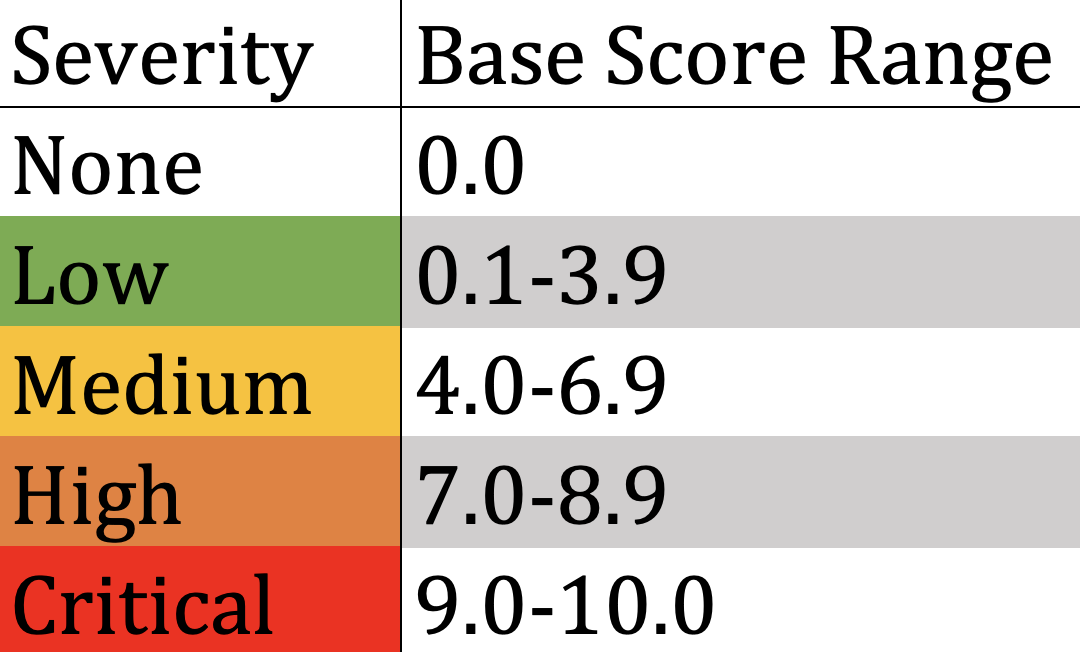
\includegraphics[scale=0.3]{Images/CVSS.png}
    \caption{CVSS v3 Ratings} Adapted from:\cite{cvssrating}
    \label{fig:CVSS v3 Ratings}
\end{figure}


\subsection{Common Vulnerabilities and Exposures (CVE)}
\acrlong{cve}\footnote{Available at: https://www.cve.org/}, known as \acrshort{cve}, is, according to their website,\textit{"a list of records each containing an identification number, a description, and at least one public reference for publicly known cybersecurity vulnerabilities"}\cite{CVE}. The CVE program's mission is to determine, describe, and categorize cybersecurity vulnerabilities that have been made public. All discovered vulnerabilities will be put into records and sent to NVD.

\subsection{Common Weakness Enumeration (CWE)}
\label{cwe}
\acrlong{cwe}\footnote{Available at: https://cwe.mitre.org/}, know as \acrshort{cwe}, is \textit{"a community-developed list of common software and hardware weakness types that have security ramifications"}\cite{CWE}. It was established to serve as a consistent benchmark for security solutions that address vulnerabilities and as a baseline for identifying, mitigating, and preventing weaknesses. CWE's goal is to provide instructions for those who have control over and maintain source code to stop the vulnerabilities at the source. 

\subsection{OWASP Risk Rating Methodology}
OWASP Risk Rating Methodology contains a formula that calculates a risk score for each vulnerability based on two factors: likelihood and impact. There are multiple factors that make up both likelihood and impact. 
 
Factors that together compose the estimation of likelihood are separated into different groups which are related to the threat actor and the vulnerability. The set of factors related to the threat actor is skill level, motive, opportunity, and size. The set of factors related to the vulnerability is the ease of discovery, ease of exploit, awareness, and intrusion detection. Each factor will have different options, and each option will receive a likelihood rating from 0-9. 

Factors that together compose the estimation of impact are divided into technical impact and business impact. The technical impact is broken down into confidentiality, integrity, availability, and accountability. Further, the business impact is divided into financial damage, reputation damage, non-compliance, and privacy violation. All of the factors will, like the factors of likelihood, receive an impact rating from 0-9. 

Combining the estimates of likelihood and impact factors produces an overall severity level of the risk, which can be classified as low, medium, or high (as shown in Figure 2.5) in order to determine its severity. These levels can be further combined to determine the final severity of the risk, as illustrated in figure 2.6.\cite{owasprisk}

\begin{figure}[H]
    \centering
    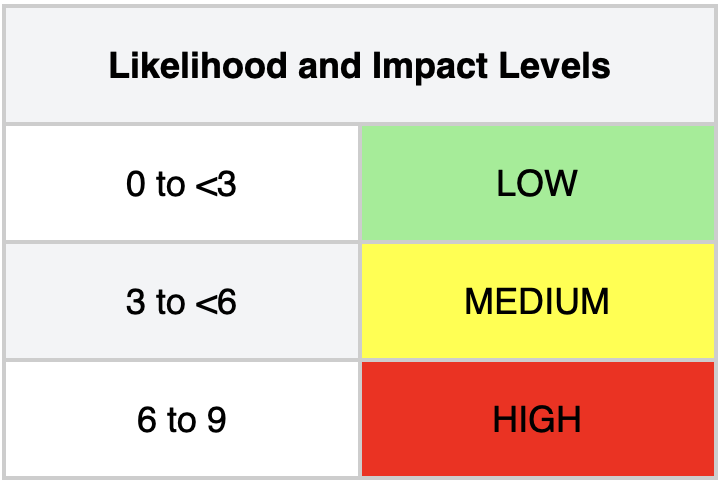
\includegraphics[scale=0.5]{Images/OWASP-likelihood.png}
    \caption{The likelihood and impact levels}
    \label{fig: Impact levels}
\end{figure}

\begin{figure}[H]
    \centering
    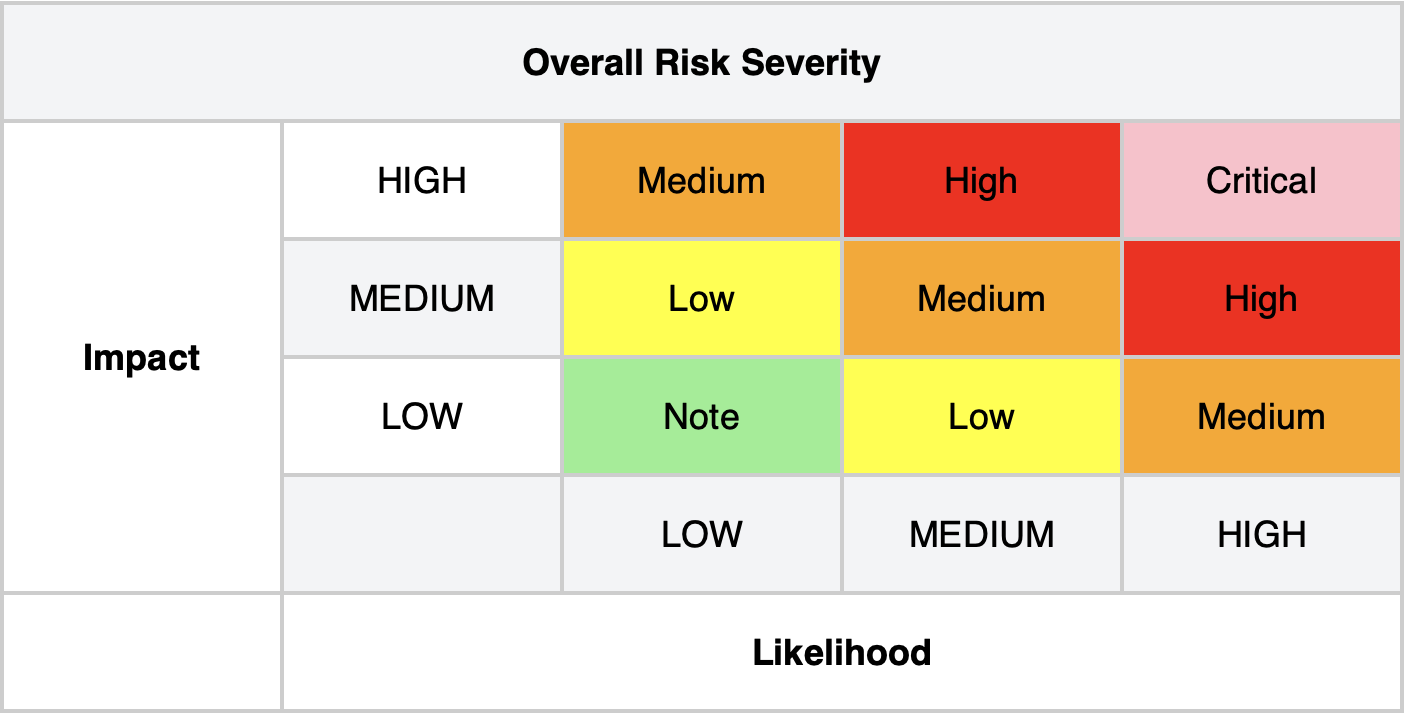
\includegraphics[scale=0.4]{Images/OWASP-severity.png}
    \caption{Severity level based on impact and likelihood}
    \label{fig: OWASP Severity Scale}
\end{figure}
\newpage




\section{Amazon Web Services}
\acrlong{aws}\footnote{Available at: https://aws.amazon.com/}, known as \acrshort{aws}, is a cloud computing platform distributed by Amazon and provides a range of services from \acrlong{iaas}(\acrshort{iaas}) to \acrlong{paas}(\acrshort{paas}), and everything in between, allowing customers to run their applications and store their data in the cloud. With their pay-as-you-go cloud computing model, the customer can scale their resources up and down - without having to invest in physical infrastructure.\cite{aws}  

\section{GitHub}
GitHub\footnote{Available at: https://github.com/} is a web-based software development platform where developers can collaborate and store open-source projects. The developers can manage their projects in repositories, and track bugs and issues. It offers a range of different collaboration tools, including pull requests, code reviews, and project management functionalities. Git is a version control system, utilized for the management and monitoring of file versioning. GitHub employs this technology as the basis for its service. This allows developers to work on code simultaneously, track changes, and merge contributions from multiple contributors.\cite{github}
